\documentclass[12pt]{exam}
\usepackage{graphicx}
\usepackage{amsfonts}
\usepackage{pgfplots}
\pgfplotsset{compat=1.18}
\usepackage{amsmath}
\usepackage{float}
\usepackage{booktabs}
\usepackage{mdframed}
\printanswers% 
\setlength{\parindent}{0cm}
\usepackage{tikz}
\usetikzlibrary{shapes.geometric, arrows.meta, positioning}
\usepackage[backend=biber,style=numeric]{biblatex}
\addbibresource{refs.bib}
\usepackage{etoolbox}
\patchcmd{\abstract}{\quotation}{\noindent\ignorespaces}{}{}

\newtheorem{example}[subsection]{Example}
\newtheorem{thm}[subsection]{Theorem}
\newtheorem{defn}[subsection]{Definition}
\newtheorem{prop}[subsection]{Proposition}
\newtheorem{claim}[subsection]{Claim}
\newtheorem{cor}[subsection]{Corollary}
\newtheorem{lemma}[subsection]{Lemma}


\title{Topological Data Analysis in Image Processing}
\author{Jakob Rode, West, Marko}
\date{June 2025}

\begin{document}

\maketitle



\begin{abstract}
\noindent   

In this paper, we will summarize some recent advancements in the intersection of topological data analysis and image processing and then proceed to our own case study. We will establish the necessary mathematical background, examine various medical and scientific applications, and discuss the differences and similarities between TDA and more traditional machine learning methods. We have compiled a dataset of cartoon characters on which we will demonstrate some of the methods discussed in the paper using python and the gudhi library.
\end{abstract}
\newpage

\section{Introduction}

Over the last few decades, the field of topological data analysis has emerged in order to understand increasingly complex and high-dimensional data. TDA provides tools to extract meaningful geometric and topological features, such as connected components, loops, and holes from data, without relying on predefined coordinates or metrics. Put simply, it allows one to study the "shape" of data.  \\

While topology, and in particular algebraic topology, the mathematical background of TDA has been around for over a century, applying these rigorous methods to real data is still a fairly new concept. Some of the early pioneers of the field include Herbert Edelsbrunner and Gunnar Carlson in the early 2000's with the formulation of the persistence diagram, and it's intuitive visualizations as persistence diagrams and barcodes. Today, although still in its infancy, TDA is accepted as a useful tool in the scientific community for analyzing complex high dimensional point clouds. Modern imaging technologies generate vast amounts of high-dimensional, often noisy data that challenge conventional analysis techniques. From medical scans and microscopy to satellite and materials imaging, the task of extracting robust, meaningful features from complex image structures is a task well suited for topological data analysis. 

\section{Mathematical Background}

The mathematics underlying topological data analysis are advanced and mostly out of the scope of this paper, however we will define a few of the most important concepts.  \\



Let \( V \) be a finite set of vertices. A \(k\)-simplex is  denoted as the set
\[
\sigma = \{v_0, v_1, \ldots, v_k\} \subseteq V
\]
where each subset of \( \sigma \) is also a face of the simplex. A simplicial complex \( K \) over \( V \) is a collection of simplices such that:
\begin{enumerate}
    \item If \( \sigma \in K \), then every face \( \tau \subseteq \sigma \) is also in \( K \),
    \item Every vertex of \( \sigma \in K \) belongs to \( V \).
\end{enumerate}

A widely used construction is the Vietoris–Rips complex. Given a finite  point cloud \( X \subseteq \mathbb{R}^n \) and a scale parameter \( \epsilon > 0 \), the Vietoris–Rips complex \( \mathrm{VR}_\epsilon(X) \) contains a \( k \)-simplex for each subset of \( k+1 \) points whose pairwise distances are all \( \leq \epsilon \). A filtration is a nested sequence of simplicial complexes built from data, where each complex $K_\epsilon$ includes more simplices as the scale parameter $\epsilon$ increases. \\



Let \( \{K_\epsilon\}_{\epsilon \geq 0} \) be a filtration of simplicial complexes:
\[
K_0 \subseteq K_{\epsilon_1} \subseteq K_{\epsilon_2} \subseteq \cdots \subseteq K_{\epsilon_n}
\]

For each scale \( \epsilon_i \), we construct a simplicial complex \( K_{\epsilon_i} \) from the data and examine its topological features—such as the number of connected components, loops, or enclosed voids. As \( \epsilon \) increases, more connections form between data points, causing new features to appear and existing ones to disappear. \\

Persistent homology tracks these features across the entire sequence of scales. If a feature appears at scale \( \epsilon_i \) and disappears at scale \( \epsilon_j \), we record this with a persistence interval:
\[
[b, d) \quad \text{where } b = \epsilon_i, \ d = \epsilon_j
\]

These intervals are collected into a persistence barcode or a persistence diagram, which visually summarize the lifespan of topological features across scales. Features that persist over a large range of \( \epsilon \) are typically considered meaningful, while short-lived features are often treated as noise. \\

This is far from a complete study of the mathematics behind topological data analysis, but it does lay some of the groundwork to contextualize the content of this paper.

\section{From Images to Point Clouds}

In this paper, we want to apply TDA techniques to the processing of images. In order to do this however, we need to encode our image as a point cloud, which in its own is not a trivial task. A picture taken with a digital camera is generally stored as a two dimensional array where the values are either RGB values (color images) or pixel intensities (grayscale images).  \\

The most natural way to embed a grayscale image is to consider $\{(x, y, I)\} \subset \mathbb{R}^3$ where $x, y$ are the array indices and I is the grayscale intensity. Similarly for an RGB image we may encode it as $\{(x, y, R, G, B)\} \subset \mathbb{R}^5$ \\

Additionally we may discretion our intensity values to binary values, down sample by picking every $n$-th pixel or using a uniform random sample, or compute graph based embeddings of the image.  \\

If we are working with a whole collection of images however, we may want to consider each image as a single point in the high dimensional space $\mathbb{R}^{m^2}$ for an image of $m * m$ image. For example, a $16*16$ grayscale image becomes a vector in $\mathbb{R}^{256}$ by flattening the 2D array into a 1D vector, where each array element corresponds to a pixel intensity. \\

These are just a few methods for encoding our images as point clouds in order to process them for topological data analysis. In practice, the method once chooses is highly contextual and depends on the particular application or problem one is trying to solve.

\section{Satellite Cloud Imaging Case Study}

In this section, we will summarize the methods used by Ver Hoef L, Adams H, King EJ and Ebert-Uphoff to classify meoscale clouds. The ability to efficiently classify cloud types is an important problem in environmental sciences that can be directly applied to weather prediction and climate monitoring models. Using traditional methods, this can be challenging due to a lack of well-labeled data sets. In this study, the authors aim to use TDA techniques on a dataset of 100,000 images to classify four different cloud meoscale cloud types, sugar, flower, fish or gravel.  The images are originally in RGB form, but the authors aim to simplify the dataset by converting to grayscale using the formula
\[
I = 0.299R + 0.587G + 0.144B
\]
which is a common method for measuring percieved brightness of an RGB image as grayscale. In order to further reduce computational complexity, the authors randomly sample six $96 * 96$ pixel subsets from each annotated image. For every subsample, the authors compute the superlevelset persistent homology in $0$ and $1$ dimensions, which are then vectorized as a point in $\mathbb{R}^{2000}$. Then the six points for an annotated image are averaged in order to obtain a single embedding for each annotation. These vectors then serve as the inputs for a support vector machine based classifier. By projecting the SVM's decision boundaries back into the topological space, the study identifies which topological features distinguish different cloud patterns. For instance, sugar clouds exhibit numerous small, bright components against a dark background, leading to prominent 0-dimensional features. \\

The results are quite impressive. The TDA-based method effectively differentiates between certain cloud types (e.g., sugar vs. flowers) but struggles with others (e.g., fish vs. flowers), likely due to the scale of distinguishing features relative to the subsample size. \\

This approach is computationally efficient as we are just taking small samples of the large dataset, requires significantly fewer labeled samples compared to deep learning methods and the method's deterministic nature allows for predictable behavior and understanding of failure modes. The study clearly shows the power of persistent homology in extracting textural differecnes in sattelite imaging. 



\section{TDA in neural circuits case study}
	In this section we will look at another use case of persistent homology in modeling connections in the brain. We summarize the techniques used and findings of Di Liang, Shengxiang Xia, Xianfu Zhang, and Weiwei Zhang in "Analysis of Brain Functional Connectivity Neural Circuits in Children With Autism Based on Persistent Homology." Autism spectrum disorder (ASD) is a complex neurodevelopmental disorder, with unclear pathogenesis, or the mechanisms which cause ASD. New methods are emerging to classify physical differences in the brain of people with ASD and without. The researchers in this paper used resting-state functional magnetic resonance imaging (fMRI) along with construction of Vietoris-Rips filtrations to analyze the difference in the number of FC neural circuits of different length ranges between people with ASD and without. \\

	To do this, they first extracted fMRI time series for 90 brain regions, using the AAL atlas. Functional connectivity between each pair of regions in the brain were then quantified using the pearson correlation coefficient, resulting in a symmetric correlation matrix for each subject. The distance metric $d(P_i,P_j) = \sqrt{1-\text{corr}(P_i,P_j)} $ was defined using the correlation coefficient to determine the distance between vertices in the brain functional network. \\

	For each subject's FC matrix, a VR-complex filtration was built by varying the threshold parameter based on the distances in the correlation matrix. This results in the VR-filtration model of the brain network:
	\[
	\text{VR}(X,\ep_1) \subset \text{VR}(X,\ep_2) \subset  \ldots
	.\] 
Using JavaPlex, they then calculated the persistence barcodes and 0 and 1 dimensional Betti numbers. These can be interpreted to be the number of connected components of the brain network, and the number of functional circuits in the brain network, respectively. \\

To analyze the results from the filtrations, persistence barcodes across thresholds 0.7,0.8, and 0.9 were used to count the number of FC neural circuits of different lenghts in the typical vs ASD individuals. Then statistical comparisons using the Mann-Whitney U-test wer applied to the length ranges of 4-7, 8-12, and 13-16. They found that the number of circuits of length 8-12 was significantly lower in ASD children, while no significant difference was found for very short or long circuits. Also, when the threshold is 0.7, the ASD group had 7 connected components, while in the TD control, all brain regions were connected, forming 1 component. \\

These results gained from the techniques learned from persistent homology give us important insights into the connections between brain regions in people with ASD, and help model the features of the brain which may influence its functions. 




\section{Cartoon Characters and TDA}

In this section, we now move on to our own example where we apply a few basic TDA methods on a dataset we compiled of about 200 images of cartoon characters


\subsection{The topology of Homer Simpson}

\begin{mdframed}
\centering
\begin{minipage}{0.18\linewidth}
    \centering
    \includegraphics[width=\linewidth]{homer.jpg}
\end{minipage}
\hfill
\begin{minipage}{0.6\linewidth}
    \centering
    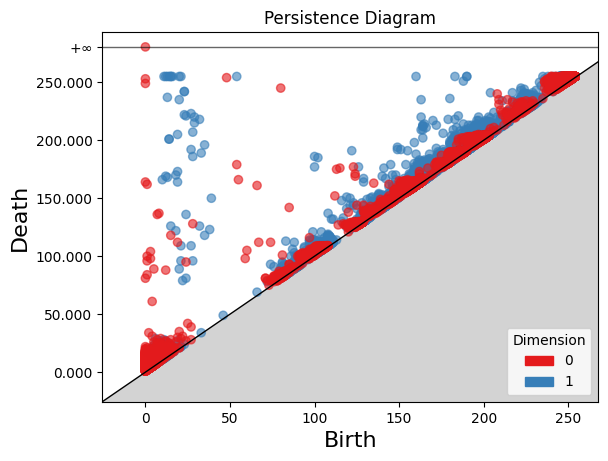
\includegraphics[width=\linewidth]{homer_pd.png}
\end{minipage}
\end{mdframed}


\end{document}
